\section{Filter design}

\subsection{Analoge filtre}

Det analoge filter design har blandt andet funktionen at isolerer og forstærke DC niveauet fra tryksensoren, som er koblet til manchetten. Tryksensoren (MPX5100) er lineær og kan derfor ud fra en enkel koefficient kalibreres.1 DC niveauet skal forstærkes for at øge ADC opløsningen i forhold til mmHg per bit. Arduino MEGA 2560 har en ADC opløsning på 10bit. I volt er dette en opløsning på 5/1023=4.9mV. Sensoren har en sensitivitet på 45mV/kPA, svarende til 6mV/mmHg. Uden DC forstærkning er opløsningen altså 4.9/6=0.817mmHg. Ved at anvende gain X2 øges opløsningen til 0.817/2=0.408mmHg. Ren DC opnås ved at lavpas filteret fjerner alt AC over knækfrekvensen.

\begin{figure}[H]
	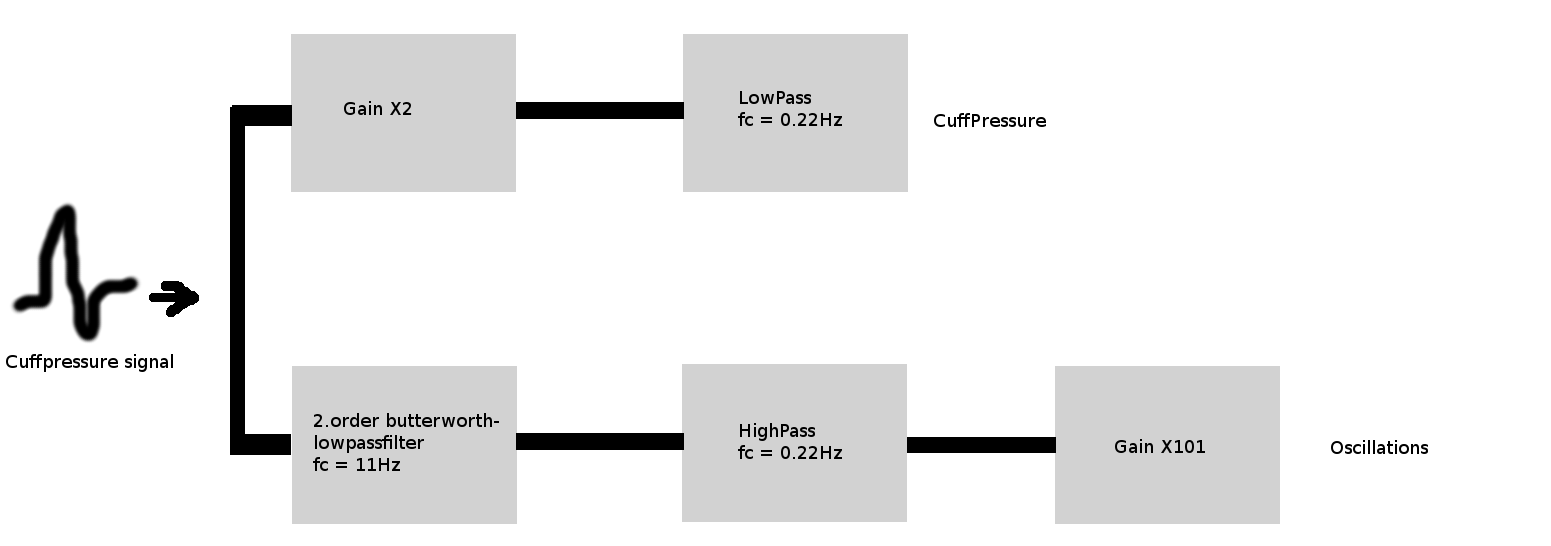
\includegraphics[width=\textwidth]{billeder/AnalogFilter.png}
	\caption{Filter model med inputsignal til venstre og de to output signaler	til højre}\label{pic:analogfilter}
\end{figure}
CuffPressure er forstærket DC og Oscillations er forstærket AC mellem 0.22Hz og 11Hz

Oscillationerne i manchetten isoleres med 11Hz anden ordens butterworth for at opnå god dæmpning på 50Hz brummen. L.A. Geddes et al. Sætter knæk frekvensen til 30Hz2, men efter som at puls signalet befinder sig på ca 1Hz og at Geddes med høj sandsynlighed har anvendt kaskade filtre sættes butterworth filterets knæk til 11Hz, svarende til elve afledte af puls grund frekvensen. Højpasfilteret fjerner DC ved at knække ved 0.22Hz. For at forstærke oscillationerne op i en størrelse, som arduinoen kan sample forstærkes det pulserende signal med gain X101.

\subsection{Komponent udregninger}
\textbf{INDSÆT MAPLE REFERENCE}

\subsection{Praksis}
Signal generator med frekvens 0.8Hz svarende til en sund puls. Simuleringen er vist på billederne under. Den lilla kurve er inputsignalet, rød er det oscillerende udgangssignal efter filteret og den grønne kurve er udgangssignalet efter det ikke oscillerende filter.

\begin{figure}[H]
	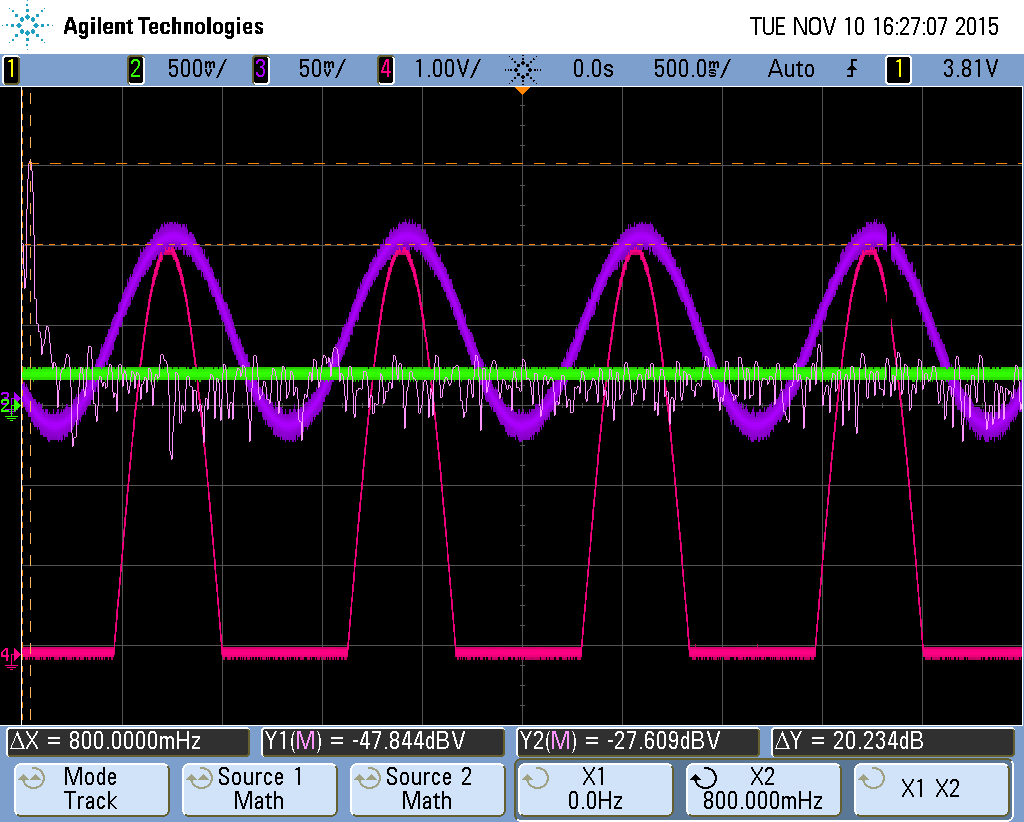
\includegraphics[width=\textwidth]{billeder/scope_9.png}
	\caption{Lilla er input sinus 0.8Hz. Grøn er ren DC. Rød er det filtrerede signal med oscillationerne. Den lyserøde kurve er FFT af det lella signal, hvor det ses at det består af 0.8Hz grundtone.}\label{fig:filterone}
\end{figure}

\begin{figure}[H]
	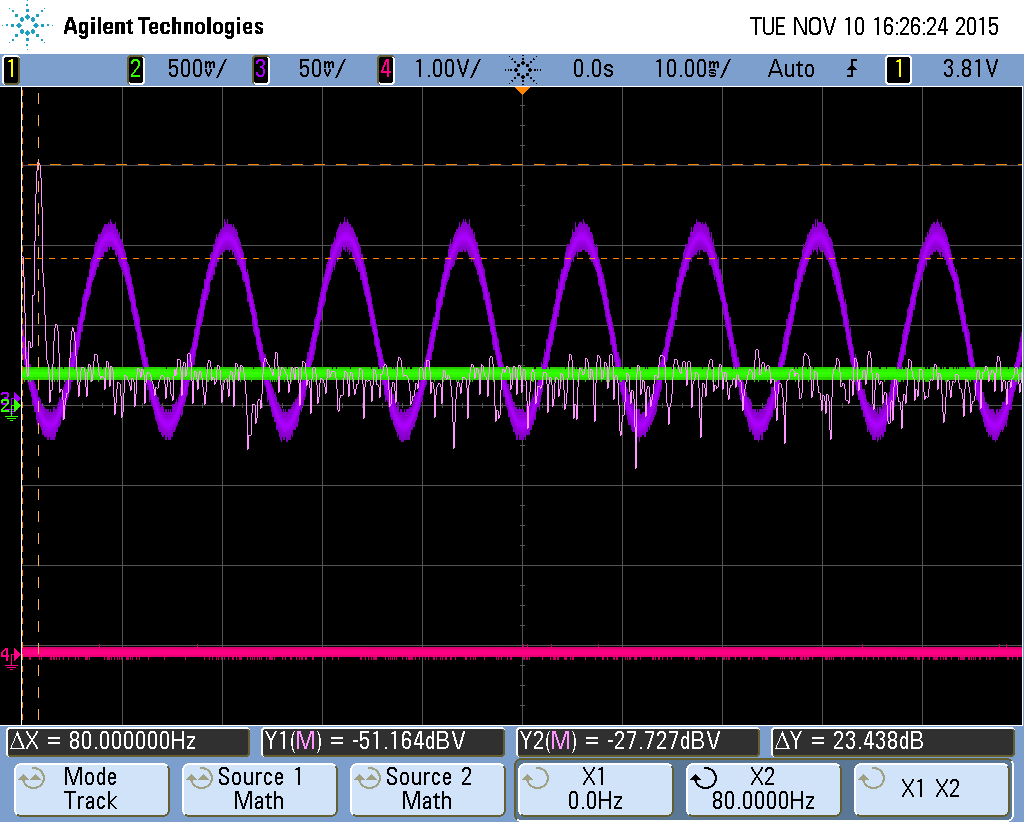
\includegraphics[width=\textwidth]{billeder/scope_8.png}
	\caption{Lilla er input sinus 80Hz. Grøn er ren DC. Rød er det 	filtrerede signal med oscillationerne. Den lyserøde kurve er FFT af det lella signal, hvor det ses at det består af 80Hz grundtone.}\label{fig:filtertwo}
\end{figure}
\newpage

\begin{figure}[H]
	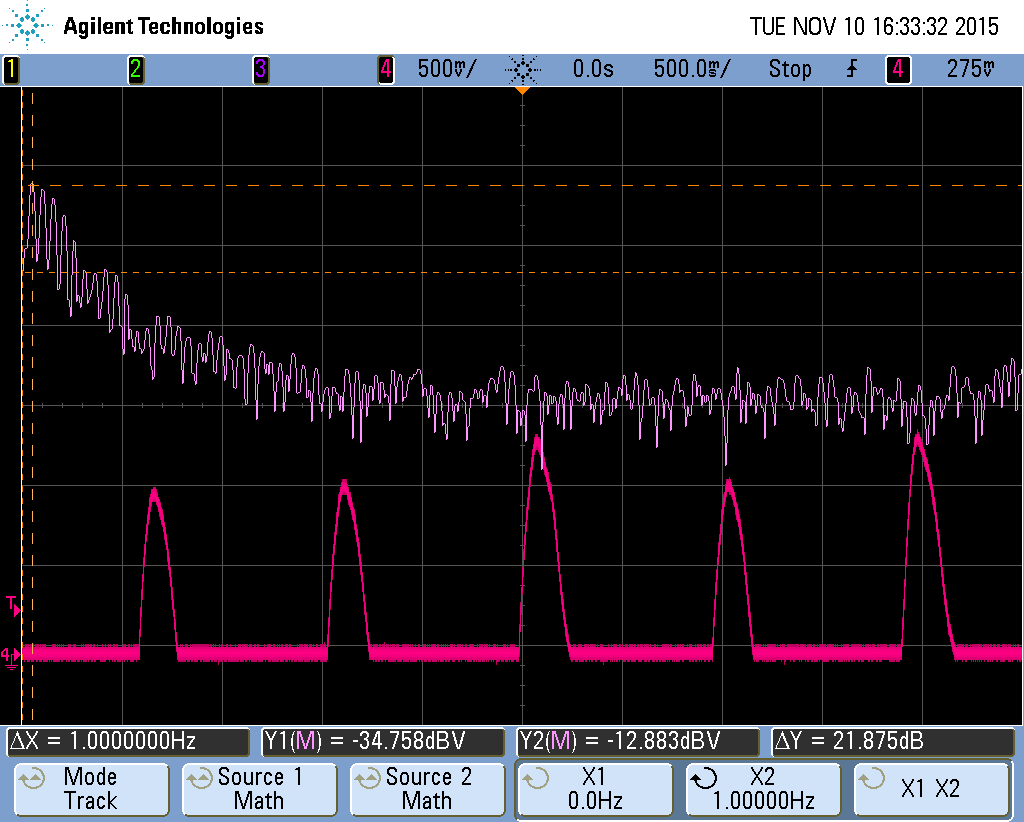
\includegraphics[width=\textwidth]{billeder/scope_10.png}
	\caption{Oscilloskop billedet viser udgangssignalet efter den oscillerende 	filtrering (Rød) og en FFT af signalet (lyserød). Her ses det tydeligt at grundtonen er ca 1Hz og har mindst 4 afledte der af 	(2,3,4,5 Hz), som gider den spidse smalle form.}\label{fig:filterthree}
\end{figure}

Hvis manchet signalet ikke simuleres, men i stedet måles på et rigtigt menneske ligner signalet ikke perfekte sinuser, men i stedet korte udsving, med en grundfrekvens og en masse overtoner. På nedenstående billede ses forskellige typiske udgangssignaler under en normal blodtryksmåling.
\newpage

\begin{figure}[H]
	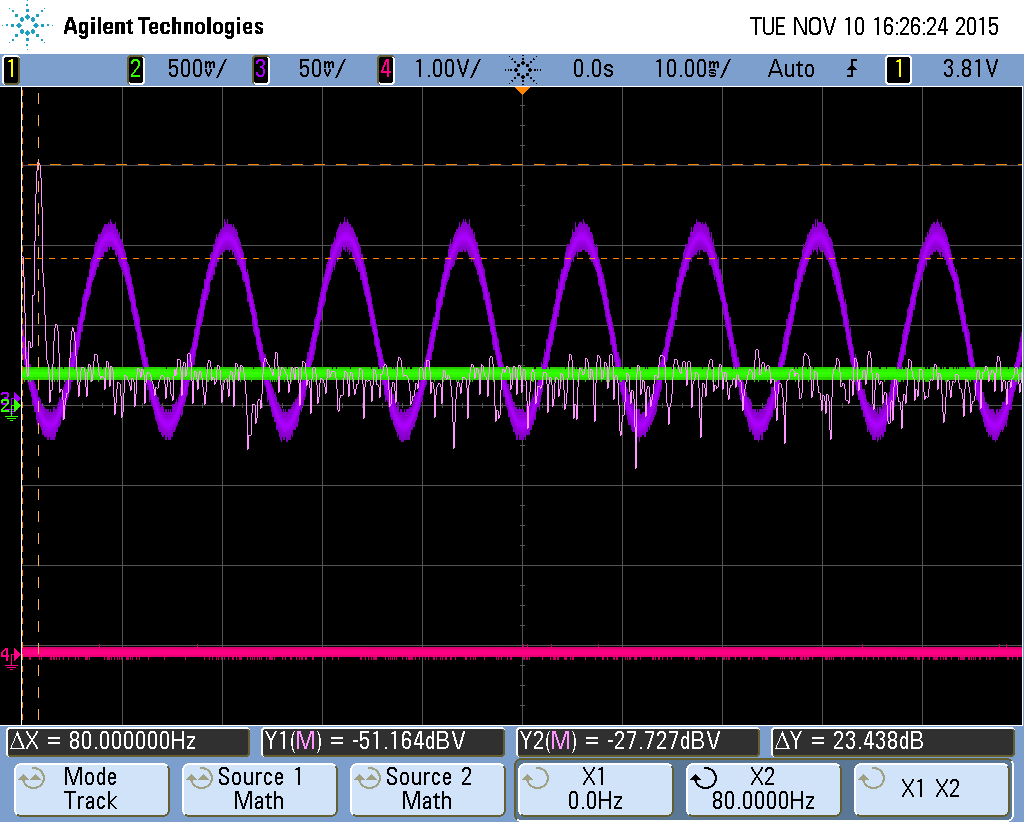
\includegraphics[width=\textwidth]{billeder/scope_8.png}
	\caption{Når manchet trykket nærmer sig det systolliske tryk obesrveres 	der et signal som ser lidt anderledes u.}\label{fig:filterfour}
\end{figure}

Det ses meget tydeligt på billede (XX og XX) at det pulserende signal svinger meget med hensyn til peak amplituden over tid. Dette fænomen ses kan sskyldes mange ting, her iblandt respirationen og andre mekaniske bevægelse. Den analoge filtrering når sin begrændsning, da den ikke kan filtrere peak amplituden til at passe en optimal blodtryksmåling, som kan ses på figur XX, hvor amplituderne er konstant stigende ind til MAP og så aftagende efterfølgende. Til at håndterer dette problem anvendes der digital filtrering.
\newpage

\begin{figure}[H]
	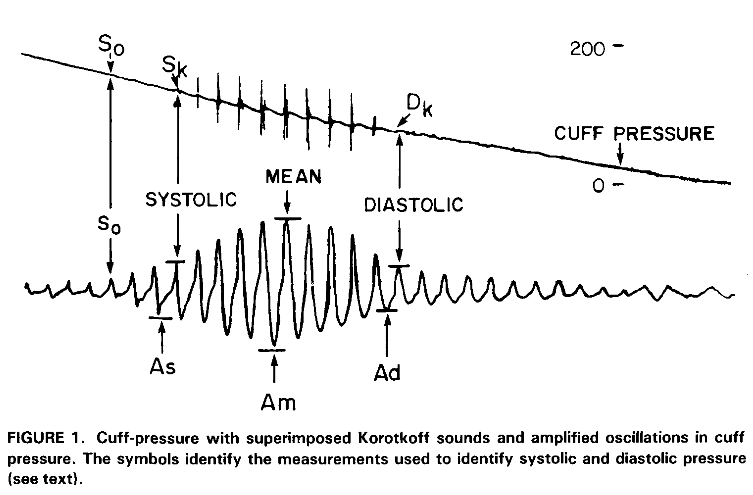
\includegraphics[width=\textwidth]{billeder/OptimalBlodtryksmaling.png}
	\caption{Billedet er taget fra CHARACTERIZATION 	 OF THE OSClLLOMETRlC METHOD FOR MEASURING INDIRECT BLOOD 	PRESSURE}\label{fig:goodMeasurement}
\end{figure}

\subsection{Digital filtrering}
Til digital filtrering er der anvendt et ekspotentiel midlingsfilter med zero group delay.
y(n) = ax(n)+(1-a)y(n-1)
Filteret midler peak ampletryderne, så den gennemsnitlige ampletyde forøgelse/dæmpning kommer til udtryk. Blodtryks filteret anvender en alfaværdi på a = 0.11. Udermere filtreres data fra begge sider, altså først fra venstre mod højre og så bag efter fra højre mod venstre. Denne teknik sikre ingen group delay, som er vigtigt for at kunne bestemme MAP, som det tryk der er i manchetten på samme tidspunkt som den maksimal målte peak ampletyde. Dette er bedst ilistreret på figur XX, hvor manchettrykket er faldende over tid og peak amplituderne er stigende og efter MAP så faldende. Når det rå signal midles fra venstre mod højre opstår et group delay på peak ampletyderne, som ikke er på manchet tryk data'en. Af denne grund må der ikke være group delay på signalet.

\textbf{INDSÆT BILLEDE}


